\documentclass[a4paper]{article}
\usepackage[margin=.8in]{geometry}
\usepackage{indentfirst}
\title{Sorting Networks of Logarithmic Depth:\\ A Report on an AI-Assisted Research Project}

\author{}

\usepackage{amssymb,amsmath,amsthm}
\usepackage{enumerate}
\usepackage{hyperref}
%\usepackage{cite}
\usepackage[capitalize]{cleveref}
\usepackage{enumitem}
\usepackage{color}
\usepackage{cancel}
\usepackage[all, cmtip]{xy}
% \usepackage{bbm}
\usepackage{tikz}
\usetikzlibrary{shapes}
\usepackage{svg}
\usepackage{import}
\usepackage{optidef}

\usepackage[utf8]{inputenc} % allow utf-8 input
\usepackage[T1]{fontenc}    % use 8-bit T1 fonts
\usepackage{hyperref}       % hyperlinks
\usepackage{url}            % simple URL typesetting
\usepackage{booktabs}       % professional-quality tables
\usepackage{amsfonts}       % blackboard math symbols
\usepackage{nicefrac}       % compact symbols for 1/2, etc.
\usepackage{microtype}
\usepackage{multirow}
\usepackage{xfrac}
%\usepackage{todonotes}
\usepackage{titlesec}
\usepackage{caption}
\usepackage{subcaption}
\usepackage{amsmath} 
\usepackage{float}
\usepackage{algorithm}
\usepackage{algpseudocode}
\usepackage{multicol} 
\newtheorem{assumption}{Assumption}

\titleformat{\subsubsection}
{\normalfont\normalsize\bfseries}{\thesubsubsection}{1em}{}
%\let\subcaption\relax
%\let\subfloat\relax
%\usepackage{subcaption}

% % Options for pgfplots
% \pgfplotsset{compat=1.12}
% \pgfplotsset{
% every x tick label/.append style={font=\footnotesize},
% every y tick label/.append style={font=\footnotesize}}
% \usetikzlibrary{pgfplots.groupplots}

% graphics for images
\usepackage{graphicx}

% If you uncomment the following line, make sure to uncomment the figures
% in the experiments section and comment the ones used now
%\usetikzlibrary{external}
%\tikzexternalize[prefix=figures/]
%\pgfkeys{
%    /tikz/external/mode=list and make
%}

%\usepackage{url}
\usepackage{appendix}
\numberwithin{equation}{section}
%%%%%%%%%% Math %%%%%%%%%%%%%%%

\newcommand{\tr}{\mathrm{Tr}}
\newcommand{\vect}{\mathbf{vec}}
\newcommand{\sym}{\R_{sym}}
\newcommand{\psd}{\cS_{+}}
\newcommand{\variety}{\mathcal{V}}
\newcommand{\cI}{\mathcal{I}}
\newcommand{\cX}{\mathcal{X}}
\newcommand{\cB}{\mathcal{B}}
\newcommand{\cE}{\mathcal{E}}
\newcommand{\ip}[1] {\langle #1 \rangle }
\newcommand{\norm}[1]{\left \| #1 \right \|}
\newcommand{\opnorm}[1]{\norm{#1}_{\mathrm{op}}}
\newcommand{\inclu}[0] {\ar@{^{(}->}}
\newcommand{\conn}{{\scriptstyle \#}}
\newcommand{\Aut}[1] {\text{Aut}_{#1}}
\newcommand{\Rank}{\text{Rank }}
\newcommand{\by}{\times}
\newcommand{\mb}{\mathbf}
\newcommand{\Ker}{\text{Ker }}
%\newcommand{\vec}{\text{Vec }}
\newcommand{\Dim}{\text{dim }}
\newcommand{\spann}{\text{span}}
\DeclareMathOperator*{\Span}{span}
\newcommand{\im}{\text{Im }}
\newcommand{\gph}{{\rm gph}\,}
\newcommand{\diag}{{\rm diag}}
\newcommand{\dist}{{\rm dist}}
\newcommand{\gap}{gap}
\newcommand{\R}{\mathbb{R}}
\newcommand{\Z}{\mathbb{Z}}
\newcommand{\N}{\mathbb{N}}
\newcommand{\CC}{\mathbb{C}}
\newcommand{\cA}{\mathcal{A}}
\newcommand{\cU}{\mathcal{U}}
\newcommand{\cS}{\mathcal{S}}
\newcommand{\fS}{\mathfrak{S}}
\newcommand{\cR}{\mathcal{R}}
\newcommand{\cN}{\mathcal{N}}
\newcommand{\mh}{\mathfrak{h}}
\newcommand{\EE}{\mathbb{E}}
\newcommand{\trace}{\mathrm{Tr}}
\newcommand{\sign}{\mathrm{sign}}
\newcommand{\lip}{\mathrm{lip}}
\newcommand{\var}{\mathrm{var}}
\newcommand{\Var}{\mathrm{Var}}
\newcommand{\RR}{\mathbb{R}}
\newcommand{\B}{\mathbb{B}}
\newcommand{\C}{\mathbb{C}}
\newcommand{\PP}{\mathbb{P}}
\newcommand{\pfail}{p_{\mathrm{fail}}}
\newcommand{\rank}{\mathrm{rank}}
\newcommand{\supp}{{\mathrm{supp}}} % support
\newcommand{\op}{\mathrm{op}}
\newcommand{\eqd}{\stackrel{d}{=}}
\renewcommand{\SS}{{\mathbb{S}}}
\newcommand{\FF}{{\mathbb{F}}}
\newcommand{\F}{{\mathbb{F}}}
\newcommand{\cF}{{\mathcal{F}}}
\renewcommand{\P}{\mathbb{P}}
\newcommand{\U}{\text{U}}
\newcommand{\SU}{\text{SU}}
\newcommand{\SO}{\text{SO}}
\newcommand{\St}{\text{St}}
\newcommand{\OO}{\text{O}}
\newcommand{\re}{\text{Re}}
\DeclareMathOperator*{\conv}{conv}
\DeclareMathOperator*{\str}{str}
\newcommand{\SPAN}{\text{span}}
\newcommand{\Diag}{\text{Diag}}


\newcommand{\pard}[2]{\frac{\partial #1}{\partial #2}}
\newcommand{\abs}[1]{\left| #1 \right|}
\newcommand{\todo}[1]{{\color{red}#1}}

%%%%%%%%% Convex Analysis %%%%%%%%%
\newcommand{\prox}{\text{prox}}
\newcommand{\proj}{\mathrm{proj}}
\newcommand{\dom}{\text{dom}}
\newcommand{\epi}{\text{epi }}
\newcommand{\hypo}{\text{hypo }}
\newcommand{\argmin}{\operatornamewithlimits{argmin}}
\newcommand{\argmax}{\operatornamewithlimits{argmax}}
\newcommand{\ls}{\operatornamewithlimits{limsup}}
\newcommand{\NN}{\mathbb{N}}
%%%% Probability %%%%%%%%%%%%%%%%%
\newcommand{\Expect}{\mathbb{E}}
\newcommand{\Prob}[1]{\mathbb{P}\left( #1 \right)}
\newcommand{\Expec}[1]{\mathbb{E}\left( #1 \right)}
\newcommand{\matrx}[1]{\begin{bmatrix} #1 \end{bmatrix}}
%%%%%%%% Theorems %%%%%%%%%%%%%
\newtheorem{thm}{Theorem}[section]
\newtheorem{theorem}{Theorem}[section]
\newtheorem{conjecture}{Conjecture}[section]
\newtheorem{definition}[thm]{Definition}
%\newtheorem{proposition}[thm]{Proposition}
\newtheorem{lemma}[thm]{Lemma}
\newtheorem{cor}[thm]{Corollary}
\newtheorem{corollary}[thm]{Corollary}
\newtheorem{pa}{Part}
\newtheorem{subclaim}{Subclaim}
\newtheorem{question}{Question}
\newtheorem{remark}{Remark}
\newtheorem{model}{Model}
\renewcommand*{\theassumption}{\Alph{assumption}}

% Explicit names for environments
\crefname{claim}{claim}{claims}
\Crefname{claim}{Claim}{Claims}
\crefname{lem}{lemma}{lemmas}
\Crefname{lem}{Lemma}{Lemmas}
\crefname{algorithm}{algorithm}{algorithms}
\Crefname{algorithm}{Algorithm}{Algorithms}

%\newtheorem{remark}{Remark}
\newtheorem{notation}{Notation}
\newtheorem{example}{Example}[section]

\newtheorem{claim}{Claim}
%%%%%%% Notation %%%%%%
\newcommand{\cT}{\mathcal{T}}
\newcommand{\cD}{\mathcal{D}}
\newcommand{\cIs}{\cI^\mathrm{sel}}
\newcommand{\cIo}{\cI_\mathrm{out}}
\newcommand{\cIi}{\cI_\mathrm{in}}
\newcommand{\cIis}{\cIi^\mathrm{sel}}
\newcommand{\cIos}{\cIo^\mathrm{sel}}
% \newcommand{\1}{\mathbbm{1}}
\newcommand{\mmid}{\ \middle|\ }
\newcommand{\set}[1]{\left\{ #1 \right\}}

% Macros for initialization section
\newcommand{\Linit}{L^{\mathrm{init}}}
\newcommand{\Rinit}{R^{\mathrm{init}}}
\newcommand{\what}{\widehat{w}}
\newcommand{\xhat}{\widehat{x}}
\newcommand{\wbar}{{\bar{w}}}
\newcommand{\xbar}{{\bar{x}}}
\newcommand{\wstar}{{w^{\star}}}
\newcommand{\xstar}{{x^{\star}}}
\newcommand{\quant}{\mathtt{quant}}
\newcommand{\bsign}{\mathbf{sign}}
\newcommand{\med}{\mathtt{med}}
\newcommand{\Xstar}{X_{\star}}
\newcommand{\eps}{\varepsilon}
\newcommand{\deltanc}{\Delta_f}

% notation for standard normal RVs
\newcommand{\normal}{\mathrm{N}}

\usepackage{mathtools}
\DeclarePairedDelimiter{\dotp}{\langle}{\rangle}

\usepackage[T1]{fontenc}
\usepackage{lmodern}


\newcommand{\comp}[3]{\draw[thick] (#1,-#2) -- (#1,-#3); \fill (#1,-#2) circle (2pt); \fill (#1,-#3) circle (2pt);}
\newcommand{\Dmerge}{D_{\mathrm{mrg}}}

\begin{document}
\maketitle

\begin{abstract}
    Sorting networks are a combinatorial object describing a parallel algorithm for sorting. They have been studied both for their practical value, for example for sorting in hardware and on parallel and embedded systems, and for their theoretical interest. Ajtai, Koml\'os and Szemer\'edi showed in \cite{AKS} that there exist sorting networks which sort any list of $n$ elements in $O(\log n)$ parallel rounds of comparisons. This construction is famously impractical: even with the improved constant of Chv\'atal \cite{chvatal1992lecture}, whose variant has depth at most $1830 \log_2 n - 58657$ for $n \ge 2^{78}$, it only becomes shallower than Batcher's simple $\tfrac12 \log_2 n(\log_2 n + 1)$-depth construction once $\log_2 n$ is in the thousands. For both small and large sorting networks there is a large gap between the best known lower and upper bounds on depth. The aim of this project was to improve our understanding of this setting, with a particular eye towards simplifying and condensing the analysis of the AKS sorting network. This report describes the effort made by the team ``An Excellent Sort'' in understanding and simplifying our understanding of these sorting networks, both at the large scale level and the small scale level.
\end{abstract}

\section{Introduction}

Sorting lists is a basic task in computer science. A list $(\ell_1, \dots, \ell_n)$ of items from a totally ordered set $(S,<)$ is \emph{sorted} if $\ell_i \le \ell_{i+1}$ for each $i$. The goal of a sorting algorithm is to find a permutation of the elements of the list that results in a sorted list \cite{knuth1998art}.

Comparison-based sorting algorithms famously require $\Omega(n \log n)$ comparisons in the worst case to sort an arbitrary list of $n$ elements: each comparison has two outcomes, and the algorithm must distinguish between all $n!$ orderings, so at least $\log_2(n!) = n\log_2 n - O(n)$ comparisons are needed. Methods such as mergesort and heapsort match this lower bound in the worst case, and quicksort \cite{hoare1962quicksort} matches it on average \cite{knuth1998art}. In this sense, classical sequential sorting algorithms already achieve what is possible.

However, this is only in the setting in which comparisons must be performed one after another. If comparisons may be performed in parallel, the relevant measure is the number of parallel rounds. Understanding parallel sorting methods is not only of theoretical interest; parallel algorithms for sorting are used in low level hardware to do faster sorting for small numbers of inputs.

To illustrate how parallelism helps, recall bubble sort. It proceeds in $n-1$ rounds, and after round $i$ it guarantees that the $i$ largest elements of the list are in order and in the last $i$ positions. Round $i$ does this by iterating through the list, comparing item $j$ with item $j+1$ for $j = 1, \dots, n-i$ and swapping them if they are in the wrong order. We can illustrate this algorithm with a diagram (\cref{fig:bubble}).

\begin{figure}[h]
\centering
\begin{subfigure}{.55\textwidth}
\centering
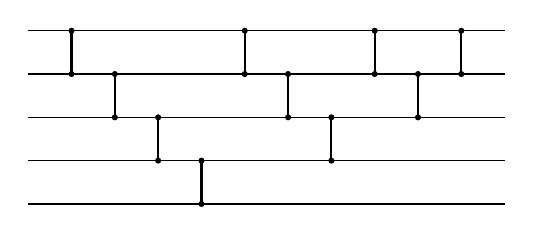
\begin{tikzpicture}[scale=.55]
\foreach \i in {0,...,4} { \draw (0,-\i) -- (11,-\i); }
\comp{1}{0}{1} \comp{2}{1}{2} \comp{3}{2}{3} \comp{4}{3}{4}
\comp{5}{0}{1} \comp{6}{1}{2} \comp{7}{2}{3}
\comp{8}{0}{1} \comp{9}{1}{2}
\comp{10}{0}{1}
\end{tikzpicture}
\caption{Bubble sort, one comparison at a time.}
\end{subfigure}%
\begin{subfigure}{.4\textwidth}
\centering
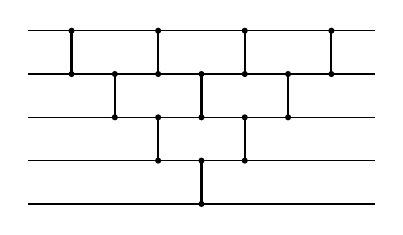
\begin{tikzpicture}[scale=.55]
\foreach \i in {0,...,4} { \draw (0,-\i) -- (8,-\i); }
\comp{1}{0}{1}
\comp{2}{1}{2}
\comp{3}{2}{3} \comp{3}{0}{1}
\comp{4}{3}{4} \comp{4}{1}{2}
\comp{5}{2}{3} \comp{5}{0}{1}
\comp{6}{1}{2}
\comp{7}{0}{1}
\end{tikzpicture}
\caption{The same comparators in $7 = 2n-3$ parallel layers.}
\end{subfigure}
\caption{Bubble sort on $n = 5$ wires as a comparator network. The first wire is at the top; each vertical gate puts the smaller of its two values on the upper wire and the larger on the lower wire.}
\label{fig:bubble}
\end{figure}

In this diagram there are $n$ horizontal wires, and we think of the items of the list as travelling along the wires from left to right. Vertical gates connect pairs of wires. Each time a pair of items reaches a gate, they are compared, and if they are in the wrong order they are swapped. The comparisons made do not depend on the input: the network is \emph{oblivious}. Note that if two gates touch disjoint pairs of wires and no gate between them touches either pair, then they can be performed in either order without affecting the result. In fact, gates that do not interact can be performed simultaneously. Thus, if we are able to operate on wires in parallel, the bubble sort network of \cref{fig:bubble}(a), which uses $\binom{n}{2}$ comparisons, can be rearranged as in \cref{fig:bubble}(b) to run in only $2n-3$ parallel rounds. (Insertion sort gives the same network after this rearrangement \cite[Section 5.3.4]{knuth1998art}.)

Formally, for $1 \le i < j \le n$ we define the comparator $C_{ij} : S^n \to S^n$ to be the map which is the identity on lists $\ell \in S^n$ with $\ell_i \le \ell_j$, and which swaps entries $i$ and $j$ if $\ell_i > \ell_j$. A \emph{comparator network} is described by a sequence of pairs $(i_t, j_t)$, $t = 1, \dots, T$, with $i_t < j_t$; it computes the composition $C_{i_T, j_T} \circ \dots \circ C_{i_1, j_1}$. It is a \emph{sorting network} if this composition maps every list to its sorted version. The \emph{size} of the network is $T$, the number of comparators. A \emph{layer} is a set of comparators on pairwise disjoint wires, and the \emph{depth} of the network is the least number $d$ such that the sequence can be grouped into $d$ consecutive layers, with comparators inside a layer applied simultaneously. Equivalently, the depth is the length of the longest chain of comparators in which each one acts on a wire used by the previous one. We write $D(n)$ for the least depth of a sorting network on $n$ wires.
Sorting networks were first studied by Bose and Nelson \cite{bose1962sorting} (following patents of O'Connor and Nelson from the late 1950s \cite[Section 5.3.4]{knuth1998art}), and were popularized by Batcher \cite{batcher1968sorting} and Knuth \cite{knuth1998art}.

For algorithmic purposes we are generally interested in constructing shallow sorting networks. Batcher \cite{batcher1968sorting} showed that a simple recursive construction, sorting the two halves of the list and merging them with a network of depth $O(\log n)$, yields sorting networks of depth $\tfrac12 \log_2 n (\log_2 n + 1)$ when $n$ is a power of $2$. These networks are of real practical value. In \cite{AKS}, it was shown that it is possible to achieve depth $O(\log n)$. Since then, several papers have attempted to simplify the techniques of \cite{AKS} and to improve the constant: Paterson \cite{paterson1990improved} gave a simplified construction with depth below $6100 \log_2 n$, Chv\'atal \cite{chvatal1992lecture} worked out a variant with depth at most $1830\log_2 n - 58657$ for $n \ge 2^{78}$, and Seiferas \cite{seiferas2009sorting} gave a further simplified analysis. On the lower bound side, the best known bound is $(3.27 - o(1))\log_2 n$, due to Kahale, Leighton, Ma, Plaxton, Suel and Szemer\'edi \cite{kahale1995lower}, improving the bound of roughly $2.41 \log_2 n$ obtained by Yao \cite{yao1980bounds}. For small $n$ the exact values of $D(n)$ are known only for $n \le 17$, by SAT-based search \cite{bundala2014optimal, codish2019end}, and the best known upper bounds for larger $n$ are collected by Dobbelaere \cite{dobbelaere}.

\section{Purpose of This Effort}
This effort had the goal of producing a simpler and clearer understanding of the AKS sorting network using AI agents from the Open Math OS models, Claude, and ChatGPT. As part of this effort, we made attempts to produce novel analysis of the AKS sorting network in particular, as well as using AI agents to attempt to produce new constructions of $O(\log(n))$ depth sorting networks that were simpler or that have connections to other areas of mathematics. We also aimed to find lower bounds on the possible sizes of sorting networks that could help explain why the AKS network has the size that it does, and also to provide simpler proofs of existing lower bounds in the literature. Finally, we aimed to see if LLMs could be used to find smaller sorting networks for fixed values of $n$.

\section{Statement of Outcomes}
We used AI agents to find the following things (with attributions to the appropriate AI service that was used to obtain the corresponding outcome).
\begin{itemize}
    \item Proofs ``by hand'' (i.e.\ without requiring the use of SAT solvers) of lower bounds for $D(n)$ for small $n$. These include an improvement to the best known lower bound for $D(32)$, from $10$ to $11$. (Claude and ChatGPT)
    \item Improved constants for AKS-style sorting networks. (Open Math Model)
    \item Improved depths for sorting networks for $n = 128$ and $n = 1024$, and verified constructions for $n = 256$ and $n = 512$ that improve on Batcher's networks. (Claude)
\end{itemize}

We attempted to develop novel perspectives on AKS-style sorting networks, but the results were not illuminating. See the attached document for an attempt at a potential function style analysis of the AKS sorting network which was ultimately not successful. We also record a number of negative results and corrections in \cref{sec:other}.

We give detailed descriptions of these outcomes below. Throughout, wires are numbered $0, \dots, n-1$, and a \emph{standard} comparator $(a,b)$ with $a < b$ puts the minimum on wire $a$. Logarithms are base $2$. Most arguments use the \emph{zero-one principle}: a comparator network sorts all inputs if and only if it sorts all inputs consisting of $0$s and $1$s \cite[Section 5.3.4]{knuth1998art}. Full proofs of everything below are in the accompanying results document.

\section{Proofs of Lower Bounds for Small \texorpdfstring{$n$}{n}}\label{sec:small}

The exact values of $D(n)$ are known for $n \le 17$ \cite{bundala2014optimal, codish2019end}:
\[
D(1), \dots, D(17) = 0, 1, 3, 3, 5, 5, 6, 6, 7, 7, 8, 8, 9, 9, 9, 9, 10.
\]
These values were obtained by large SAT computations. For larger $n$, the best lower bounds in the tables we consulted \cite{dobbelaere} came from the monotonicity of $D$, giving $D(n) \ge 10$ for $18 \le n \le 32$. The main result of this section is a short recursive inequality which improves these bounds without any computer search.

\subsection{The halving lemma}

We need two standard facts. A \emph{generalized} comparator $(p,q)$ puts the minimum on wire $p$ and the maximum on wire $q$, where $p$ and $q$ are arbitrary distinct wires; a standard comparator is one with $p < q$.

\begin{lemma}[Untangling {\cite[Exercise 5.3.4.16]{knuth1998art}}]\label{lem:untangle}
If a network of generalized comparators sorts every input, then there is a standard sorting network with the same number of comparators in each layer.
\end{lemma}

\begin{proof}[Proof sketch]
Process the comparators in order while maintaining a relabeling $\pi$ of the wires, initially the identity. For a generalized comparator $(p,q)$ let $p' = \pi(p)$ and $q' = \pi(q)$. If $p' < q'$, emit $(p',q')$. Otherwise emit $(q',p')$ and compose $\pi$ with the transposition of $p'$ and $q'$, since the two wires now hold each other's contents. The new network is standard, and its output is a fixed permutation of the output of the original. A standard network fixes the sorted input, so this permutation is the identity, and the new network sorts.
\end{proof}

\begin{lemma}[Monotonicity]\label{lem:mono}
If $m \le h$ then $D(m) \le D(h)$.
\end{lemma}

\begin{proof}
In a standard $h$-wire sorting network, put $+\infty$ on the top $h - m$ wires. A $+\infty$ on a top wire is always the maximum of its comparator, so it never moves. Deleting these wires and the comparators touching them leaves an $m$-wire sorting network of no greater depth.
\end{proof}

\begin{theorem}[Halving lemma]\label{thm:halving}
For every $n \ge 3$, $D(n) \ge D(\lceil n/2 \rceil) + 2$.
\end{theorem}

\begin{proof}
Let $N$ be a standard sorting network on $n \ge 3$ wires of depth $d$, and let $F$ and $L$ be its first two layers. Each wire touches at most one comparator of $F$ and at most one of $L$, so the graph on the wires with edge set $F \cup L$ is a disjoint union of paths and even cycles. In particular it is bipartite. Let $C$ be a colour class with $|C| \le \lfloor n/2 \rfloor$, and let $V$ be the remaining $h \ge \lceil n/2 \rceil$ wires.

Consider inputs which hold arbitrary distinct real numbers (``variables'') on $V$, and constants on $C$: put $-\infty$ on $c \in C$ if $c$ is the minimum wire of its comparator in $F$, and $+\infty$ if it is the maximum wire (either, if $c$ is idle in $F$). Every comparator in $F \cup L$ joins a wire of $C$ to a wire of $V$. In layer~1 the constants are already on the correct side of their comparators, so nothing moves. In layer~2 every comparator compares a constant with a variable. Hence no two variables are compared in the first two layers.

Whenever a variable meets a constant, the outcome does not depend on the variable's value: $-\infty$ always takes the minimum output and $+\infty$ the maximum. So the set of wires holding variables after each layer does not depend on the values of the variables, and we can follow each variable as a token. The comparators of layers $3, \dots, d$ that compare two variables form a network of generalized comparators of depth at most $d - 2$ acting on the $h$ tokens. Since $N$ sorts, the variables end up in sorted order along their final wires. Numbering the tokens by these final wires, the generalized network sorts every input of $h$ values. By \cref{lem:untangle} there is a standard $h$-wire sorting network of depth at most $d-2$, and by \cref{lem:mono}, $D(\lceil n/2 \rceil) \le D(h) \le d - 2$.
\end{proof}

Some care is needed in the last step: variables change wires when they meet constants, so one cannot simply ``delete the constant wires''. An earlier version of this argument skipped this point. Iterating the theorem down to $D(2) = 1$ gives $D(n) \ge 2\lceil \log_2 n \rceil - 1$. Combining it with the known small values gives the following bounds.

\begin{corollary}\label{cor:small}
$D(n) \ge 11$ for $25 \le n \le 32$, $D(n) \ge 12$ for $33 \le n \le 48$, and $D(n) \ge 13$ for $49 \le n \le 64$.
\end{corollary}

\begin{proof}
For $25 \le n \le 32$ we have $13 \le \lceil n/2 \rceil \le 16$ and $D(13) = 9$, so $D(n) \ge 11$. For $33 \le n \le 48$, $\lceil n/2 \rceil \ge 17$ and $D(17) = 10$. For $49 \le n \le 64$, $\lceil n/2 \rceil \ge 25$, and we apply the first case.
\end{proof}

For $18 \le n \le 24$ the lemma gives nothing new. For comparison, the best known upper bound for $n = 32$ is $14$ \cite{dobbelaere}. Computing the slack $D(n) - D(\lceil n/2 \rceil) - 2$ for $n \le 17$ shows that the lemma is tight for $n = 3, 4, 5, 6, 9, 10$ and off by one for $n = 7, 8$ and $11 \le n \le 17$.

\paragraph{Novelty.} We were not able to find this inequality stated in the literature, but it is simple enough that it may well be known. A folklore $(2 - o(1))\log_2 n$ lower bound is cited in recent work, and Knuth's Section~5.3.4 and Parberry's work on lower bounds for small sorting networks should be checked before claiming priority.

\subsection{Generalizations}

The same argument gives a family of necessary conditions on the first few layers of a candidate sorting network. Write $M(r)$ for the largest $n$ with $D(n) \le r$; the known values for $r = 0, \dots, 9$ are $1, 2, 2, 4, 4, 6, 8, 10, 12, 16$.

\begin{theorem}[$t$-layer fixing]\label{thm:fixing}
Suppose a sorting network of depth $d$ has an assignment of $\pm\infty$ to $n - h$ of its input wires such that no two of the remaining $h$ inputs are compared in layers $1, \dots, t$. Then $D(h) \le d - t$, i.e.\ $h \le M(d - t)$.
\end{theorem}

\begin{theorem}[Subcube rule]\label{thm:subcube}
Let $R_k$ be the set of $0$-$1$ vectors that can appear after $k$ layers of a sorting network of depth $d$. If $R_k$ contains a subcube of dimension $h$ (a set of vectors with $n - h$ coordinates fixed and the other $h$ free), then $h \le M(d - k)$. Moreover, layer $k+1$ must contain at least $h - M(d-k-1)$ comparators with both ends among the $h$ free wires.
\end{theorem}

The proofs follow the halving lemma: the free coordinates are tracked as tokens, and the remaining layers must sort them. The second part of \cref{thm:subcube} is useful computationally because it rules out a prefix of the network for \emph{all} possible next layers at once. We also tried a two-layer version of it, which turned out to be unsound: real optimal $16$-wire sorters violate it.

\subsection{Is \texorpdfstring{$D(32) = 11$}{D(32) = 11}?}

These rules were applied to the question of whether a depth-$11$ sorting network on $32$ wires exists. The results are partial.
\begin{itemize}
    \item Any $32$-wire sorting network whose first four layers are the hypercube prefix has depth at least $12$. This was verified by exhaustive computation by two independent agents.
    \item Of $365$ sampled five-layer prefixes starting with three hypercube layers, $364$ provably admit no valid sixth layer, and one is unresolved. However, random prefixes also tend to die at layers $5$--$6$ for $n = 12, 14, 16$, where networks of the target depth do exist. So this is not evidence that depth $11$ is impossible.
    \item An exhaustive search over all fourth layers is out of reach: there are on the order of $10^{15}$ candidates, at least $2.8 \times 10^{11}$ up to symmetry.
\end{itemize}
Proving $D(2n) \ge D(n) + 3$, even just for $n = 16$, would give $D(32) \ge 12$. We were not able to do this. A related attempt to settle whether depth $13$ is possible for $n = 32$, using a SAT encoding validated on Wang's recent depth-$13$ network for $28$ wires \cite{wang2025depth13}, was inconclusive.

\section{Improved constants for AKS-style sorting networks}\label{sec:aks}

\todo{This section should describe the improved constants found by the Open Math Model. The material below summarizes the background and what was found in the Claude sessions.}

\subsection{The scheme}

All known $O(\log n)$-depth constructions follow the same outline \cite{AKS, paterson1990improved, seiferas2009sorting}. Imagine a complete binary tree whose leaves correspond to the positions of the sorted output. Each node of the tree holds a \emph{bag} of items, which is just a set of wires. The capacity of a bag at depth $d$ at stage $t$ is $b = n \nu^t A^d$ for constants $\nu < 1 < A$. In each stage, every bag applies a constant-depth \emph{separator} (built from $\eps$-halvers, which in turn come from expander graphs). It sends a small fraction $\lambda$ of its items at each extreme up to its parent and splits the rest between its two children. The analysis tracks the \emph{strangeness} of each item, the number of levels it would have to climb to reach a bag whose interval contains its rank. It shows that items of high strangeness are exponentially rare. Since the capacities shrink geometrically, after $O(\log n)$ stages every bag is tiny and the items are sorted.

The depth is $c \log_2 n$, where $c$ is (number of stages per level) $\times$ (depth of a separator). The second factor is very large, which is why the constants in the literature are in the thousands.

\subsection{What we found}

\paragraph{A missing term in Seiferas's analysis.} Seiferas \cite{seiferas2009sorting} gives three constraints on $(A, \nu, \lambda, \eps)$ that make his invariant hold. His bound on the number of native items sent to the wrong child omits one effect: a bag's own ``small strangers'' occupy the lowest positions and can push native items across the middle. For example, with exact sorting, a bag of $100$ items containing $5$ small strangers, $50$ natives of the left half and $45$ of the right sends $5$ left-natives to the right child, although his bound gives $0$. The corrected constraint is
\[
\lambda\nu \ge 2\lambda\eps A + \frac{\lambda}{A} + \frac{\eps}{2A} + \frac{2\lambda\eps A}{1 - (2\eps A)^2} + \frac{2}{8A^3 - 2A}.
\]
His theorem and his first sample parameter point survive the correction, but his second sample point, and the optimum of his printed constraints, do not. Paterson's corresponding inequality \cite{paterson1990improved} does include this term.

\paragraph{Comparing constants.} Constants in this literature are quoted in different units, which makes comparisons difficult. For example, Seiferas's often-quoted ``$6.05$'' and ``$6.95$'' count stages, not comparator layers. Converting everything to comparator layers gives the following.
\begin{center}
\begin{tabular}{lrl}
\toprule
source & $c$ in depth $\le c\log_2 n$ & how obtained \\
\midrule
Paterson \cite{paterson1990improved} & $\approx 6100$ & literature \\
Chv\'atal \cite{chvatal1992lecture} & $\approx 1830$ (for $n \ge 2^{78}$) & literature \\
Seiferas, his sample parameters & $514{,}246$ & computed from his formulas \\
Seiferas, corrected constraints, optimized & $281{,}084$ & computed \\
same architecture, refined bookkeeping & $\approx 6{,}300$ & agent derivation, not reviewed \\
\bottomrule
\end{tabular}
\end{center}
In all cases, the constant is dominated by the cost of the separators. As concrete networks for $16 \le n \le 1024$, the AKS-style constructions we built were $1.4$ to $3.9$ times deeper than Batcher's.

\section{Improved depths for sorting networks for \texorpdfstring{$n = 128$, $256$, $512$ and $1024$}{n = 128, 256, 512 and 1024}}\label{sec:constructions}

Batcher's odd-even merge sort on $n = 2^k$ wires has depth $k(k+1)/2$. For $n = 128, 256, 512, 1024$ this is $28, 36, 45, 55$. Dobbelaere's tables \cite{dobbelaere} stop at $n = 64$, and we did not find published depths for larger $n$ other than those implied by Batcher's and by Lee and Batcher's constructions \cite{lee1995multiway}. We found the following networks.
\begin{center}
\begin{tabular}{rrrrrl}
\toprule
$n$ & Batcher & Lee--Batcher & ours & size & construction \\
\midrule
128 & 28 & 27 & \textbf{26} & 1439 & 8 sorters on 16 wires, then an 8-way merge \\
256 & 36 & 34 & 34 & 3775 & 2 sorters on 128 wires, then a 2-way merge \\
512 & 45 & 43 & 43 & 9599 & 2 sorters on 256 wires, then a 2-way merge \\
1024 & 55 & 53 & \textbf{52} & 23679 & 8 sorters on 128 wires, then an 8-way merge \\
\bottomrule
\end{tabular}
\end{center}
At $n = 128$ and $n = 1024$ the new networks beat both previous constructions by one layer. At $n = 256$ and $512$ they beat Batcher's networks but only match the value given by Lee and Batcher's formula. The entries in the Lee--Batcher column are our own arithmetic from their formula.

\subsection{Multiway merging}

Let $\Dmerge(k,m)$ be the least depth of a network that merges $k$ sorted lists of length $m$ into one sorted list. The constructions rest on the following $k$-way version of Batcher's odd-even merge, which is essentially the multiway merge of Lee and Batcher \cite{lee1995multiway}.

\begin{theorem}[Multiway odd-even merge]\label{thm:merge}
$\Dmerge(k, 2m) \le \Dmerge(k, m) + \lceil \log_2 k \rceil$.
\end{theorem}

\begin{proof}
Given $k$ sorted lists of length $2m$, merge the even-indexed elements of all lists, and in parallel the odd-indexed elements. Interleave the two results as $e_0, o_0, e_1, o_1, \dots$. Let $2^t \ge k$ and apply, for $s = 2^{t-1}, \dots, 2, 1$, the layer of comparators between positions $2i+1$ and $2i+2s$ for all $i$.

We check correctness on $0$-$1$ inputs. If list $i$ has $z_i$ zeros, its even part has $\lceil z_i/2 \rceil$ zeros and its odd part $\lfloor z_i/2 \rfloor$. So the interleaved sequence has the form $0^{2b}(01)^{\delta}1^{*}$, where $\delta$ is the number of lists with $z_i$ odd, and $0 \le \delta \le k$. A direct calculation shows that if $\delta \le 2s$, the layer with parameter $s$ produces a sequence of the same form with $\delta \le s$. Starting from $\delta \le k \le 2^t$, after the last layer ($s = 1$) we have $\delta \le 1$, and $0^{2b}(01)^{\delta}1^{*}$ is then sorted.
\end{proof}

The gain over Lee and Batcher comes from the base case. An optimal depth-$9$ sorting network on $16$ wires can be chosen with first layer $(0,1), (2,3), \dots, (14,15)$. Its remaining $8$ layers then merge $8$ sorted pairs, so $\Dmerge(8, 2) \le 8$. Since $D(16) = 9$, this is optimal. Applying \cref{thm:merge} three times gives $\Dmerge(8,16) \le 17$. So $128$ wires can be sorted by $8$ blocks of $16$ in depth $9 + 17 = 26$. Similarly $\Dmerge(8, 128) \le 26$, so $1024$ wires can be sorted in depth $26 + 26 = 52$.

\subsection{Verification}

The networks for $n = 128$ and $n = 1024$ were checked by an independent certificate checker. It reads only the flat list of layers, rediscovers the block-and-merge structure, and checks:
\begin{itemize}
    \item each $16$-wire sorter on all $2^{16}$ inputs;
    \item each base merger on all $3^8$ inputs consisting of $8$ sorted $0$-$1$ pairs;
    \item each set of cleanup layers on every $0$-$1$ input it can receive;
    \item that every comparator is accounted for.
\end{itemize}
A short induction shows that passing these checks implies that the network sorts. Six deliberately broken networks (one comparator removed each) were correctly rejected. As independent cross-checks, the $128$-wire merger was run on all $17^8 \approx 7 \times 10^9$ sorted-block inputs, and the $1024$-wire network on about $49{,}000$ further $0$-$1$ inputs, with no failures. The $256$-wire network consists of two copies of the certified $128$-wire network followed by Batcher's merge, and the $512$-wire network of two copies of the $256$-wire one followed by Batcher's merge. The merges were checked on all $129^2$ (respectively $257^2$) pairs of sorted $0$-$1$ halves, which by the zero-one principle proves that both networks sort. The whole networks were also run on $20{,}000$ random $0$-$1$ inputs and $2{,}000$ random permutations each, with no failures.

\section{Other attempts and negative results}\label{sec:other}

\subsection{Asymptotic lower bounds}

The best known lower bound on the depth of a sorting network is $(3.27 - o(1))\log_2 n$ \cite{kahale1995lower}. We attempted to improve this to $4\log_2 n$, without success. We did obtain a short self-contained proof of a weaker bound. For a wire at a given time, let $m$ be the size of the smallest set of inputs which, when all zero, force the wire to hold zero. Then for every $\alpha > 0$, after $t$ layers,
\[
\sum_{\text{wires}} m^{-\alpha} \;\ge\; n\left(\frac{1 + 2^{-\alpha}}{2}\right)^{t}.
\]
Combined with a counting argument for the last few layers, this gives Yao's bound of $(2.409 - o(1))\log_2 n$ \cite{yao1980bounds} when $\alpha = 1$, and $(3 - o(1))\log_2 n$ as $\alpha \to 0$. This potential cannot give more than $3$. We also found that an earlier reconstruction of the $3.27$ bound produced by an agent relied on a false lemma, which has a four-wire counterexample.

\subsection{Structural constraints on \texorpdfstring{$O(\log n)$}{O(log n)}-depth networks}

\begin{itemize}
    \item \textbf{Long comparators are needed until the end.} If $s_t$ is the longest comparator span in layer $t$, then $\sum_{t > \tau} s_t \ge n - 2^\tau$ for every $\tau$. So after the first $\log_2 n - 1$ layers, the remaining layers still need total span at least $n/2$. This is why AKS-type networks must keep sending items back up to the root of their tree.
    \item \textbf{Displacement alone cannot be the potential.} Let $G(\sigma) = \frac12\sum_i (\sigma(i) - i)^2$. A block of $D$ layers that shrinks $G$ by a constant factor on every input needs $D \ge \log_2\log_2 n - O(1)$. The attached document gives the stronger bound $D = \Omega(\log n)$. So a potential-function proof of an $O(\log n)$ bound needs an extra term, which plays the role of the tree level in AKS.
    \item \textbf{Halvers.} Any $\eps$-halver of depth $D$ has $\eps \ge 2^{-D}$. One built from $D$ matchings between the two halves has $\eps \ge 1/(D+1)$. Experiments suggest that such halvers leave a floor of stuck elements rather than reducing the error by a constant factor.
\end{itemize}

\subsection{A refuted design}

We investigated a ``sliding window'' design intended to replace the AKS tree with a fixed schedule of local halvers at decreasing scales. We proved that for any fixed parameters it fails to sort for large $n$, for every choice of wiring. An earlier empirical claim that it achieves depth $6\log_2 n + 12$ came from a weak adversary and was retracted.

\subsection{Errors caught}

A number of claims made by the agents during the project turned out to be wrong and were caught on review. We list them since they illustrate the kinds of errors to watch for.
\begin{itemize}
    \item A lemma used to reconstruct the $3.27\log_2 n$ lower bound is false.
    \item A proof that last-layer comparators join adjacent wires had a gap (the statement is true and published \cite{codish2015endgame}).
    \item A claimed proof that $D(12) \ge 8$ came from a bug in a search program.
    \item A two-layer pruning rule for searching for small networks was unsound.
    \item A claimed contraction rate in one AKS-style analysis was wrong.
    \item A ``reduction to square merging'' presented as new is folklore.
\end{itemize}

\section{Open problems}

\begin{enumerate}
    \item Is $D(2n) \ge D(n) + 3$? The case $n = 16$ alone would give $D(32) \ge 12$.
    \item Can $\sqrt{n}$ sorted lists of length $\sqrt{n}$ be merged in depth $O(\log n)$ by a simple network? This would give a simple $O(\log n)$-depth sorting network. Small targets: $\Dmerge(4,4) = 6$ and $\Dmerge(8,8) \le 13$ (currently $\le 14$).
    \item What is the correct form of the lemma behind the $3.27\log_2 n$ lower bound, and can it be pushed towards $4\log_2 n$?
    \item Is there a short, complete proof of an AKS-type network, including the constant-depth separators, with an explicit constant?
\end{enumerate}

\bibliographystyle{plain}
\bibliography{bib}
\end{document}
